\appendix
\chapter{Приложение А. Интерфейсная модель} \label{AppendixA}

Интерфейсная модель содержит классы и интерфейсы для взаимодействия с пользователем.

\begin{figure} [h] 
  \center
  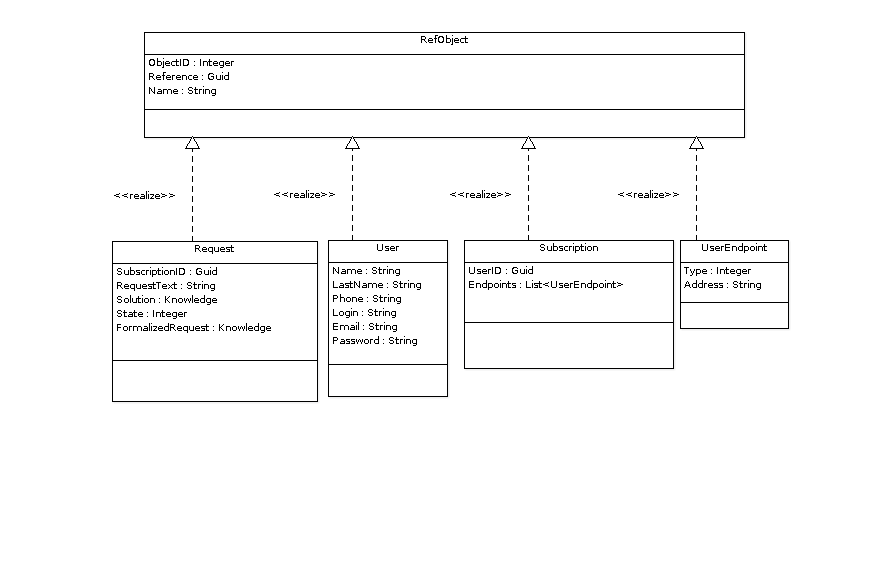
\includegraphics [scale=0.8,angle=90, origin=c] {interface-model}
  \caption{Диаграмма классов интерфейсной модели} 
  \label{img:interface-model}  
\end{figure}

\emph{RefObject}

Представляет собой общий объект, который сохраняется в Базе Знаний. (Базовый класс для всех остальных классов и объектов)
\begin{itemize}
	\item ObjectID- уникальный в пределах класса ключ
	\item Reference- уникальный в пределах всех баз знаний ключ
	\item Name-имя объекта
\end{itemize}

\emph{Request}

Объект для хранения запроса пользователя.
\begin{itemize}
	\item SubscriptionID - идентификатор подписки
	\item RequestText - запрос пользователя в виде текста
	\item Solution - ссылка на решение запроса
	\item State - статус запроса (например, Поиск Решения)
	\item FormalizedRequest - ссылка на формализованный запрос
\end{itemize}


\emph{Subscription}

Информация о подписке пользователя на события
\begin{itemize}
	\item Endpoints - списко UserEndpoint, которые будут использоваться для обратной связи с пользователем
\end{itemize}

\emph{UserEndpoint}
\begin{itemize}
	\item Type - тип точки связи с пользователем (например, веб-сервис)
	\item Address - адрес точки связи с пользователем
\end{itemize}
\clearpage

\chapter{Приложение B. Action} \label{AppendixB}
Action является базовым классом для WayToThink или Critic.
\begin{figure} [h] 
  \center
  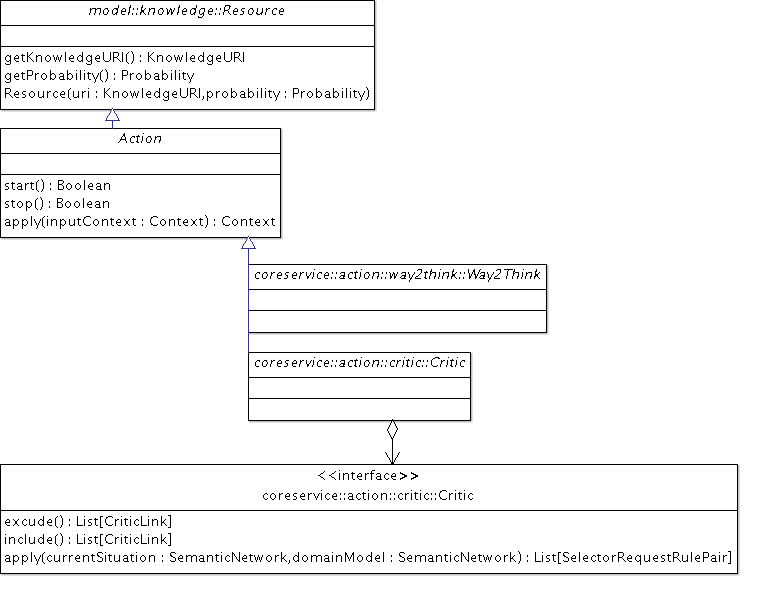
\includegraphics [scale=0.6, origin=c] {ActionClass}
  \caption{Диаграмма классов Action} 
  \label{img:ActionClass}  
\end{figure}


\chapter{Приложение C. Цели} \label{AppendixC}
Goal (Цель) является набором вероятностных предикатов и последовательностью How-To необходимых для того, чтобы достичь цель. Goal и How-To тесно связаны. На Рисунке \ref{img:goal} показан состав Goal. Goal состоит из:
\begin{enumerate}
	\item Parameters - параметры, которые используются предикатами для выполнения
	\item Precondition - условия, которые должны быть выполнены до выполнения проверок цели
	\item Entry criteria - входной критерий, предикат, который определяет, что цель активировалась
	\item Exite criteria - условия, когда цель считается выполненной
	\item PostCondition - дополнительные условия для выхода
	\item HowTo - набор решения. Список путей решения
\end{enumerate}

\begin{figure} [h] 
  \center
  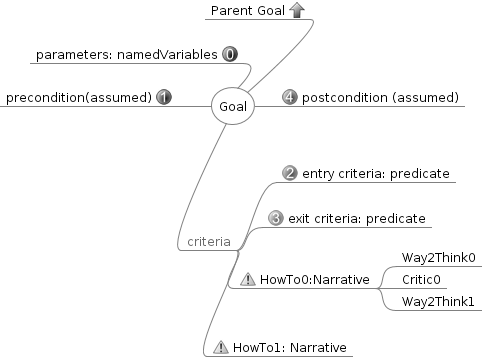
\includegraphics [scale=1.0, origin=c] {goal}
  \caption{Диаграмма классов Goal} 
  \label{img:goal}  
\end{figure}

\textbf{Типы предикатов} \\
В решение используется 3 типа логических предикатов: and, or, not. Представление Goal в SemanticNetwork показано на диаграмме \ref{img:2_0_GoalHowToConcept}.

\begin{figure} [h] 
  \center
  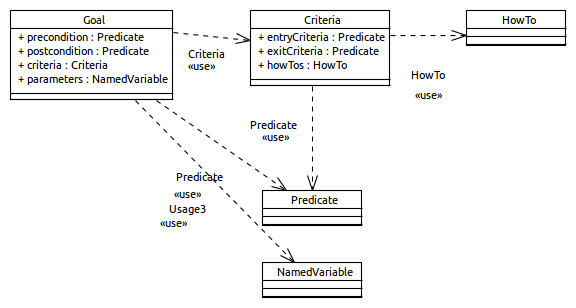
\includegraphics [scale=1.0, origin=c] {2_0_GoalHowToConcept}
  \caption{Диаграмма места Goal в SemanticNetwork (Семантической сети)} 
  \label{img:2_0_GoalHowToConcept}  
\end{figure}

Иерархия целей имеет высшую цель: Помочь пользователю. Далее вниз по иерархии идут подцели: Решить инцидент, Понять тип инцидента, Найти решение инцидента и т.д.


\chapter{Приложение D. Рецепты решений} \label{AppendixDHowTo}
Рецепты решений представляют собой последовательность действий выполняемых для решения проблемы, описанной в инциденте. 
Было разработано два типа HowTo: ValueHowTo-содержит в себе простое значение; FunctionalHowTo- содержит в себе функцию. \\
FunctionalHowTo состоит из следующих частей:
\begin{enumerate}
	\item FunctionalBody - тело функции, описывающий содержание функции
	\item InputParameters - входные параметры функции
	\item OutputParameters - выходные параметры
\end{enumerate}
Комбинация FunctionaHowTo и ValueHowTo является Рецептом Решения. Например, решение проблемы неработающего сегмента кластера в формате для специалиста технической поддержки.
\begin{itemize}
	\item Войти на сервер U1
	\item Запустить утилиту 12 для Windows Servers
	\item Открыть вкладку 1
	\item Перейти на All Managed Server, найти нужный Server из правой панели, открыть свойства сервера
	\item Нажать на Backup Exec Services
	\item Выберите проблемный сегмент кластера
	\item Нажмите Restart all Services
	\item Подождите и проверьте статус
\end{itemize}
Преобразованный в формат HowTo данный рецепт решения будет выглядеть как
\begin{lstlisting}
	
\end{lstlisting}

login:howto{
  Parameters:[

    {Key:'ScriptName',
    Value:'LogonScript.bat'},
    {Key:'Description',
    Value:'Logon to server'}
  ]

  InputParameters:[
    {Key:'ServerName',
    Value:'U1'},
    {Key:'UserName',
    Value:'MyUser'}
  ]

  OutputParameters:[
    {Key:'SessionID',
    Value:'SSSE12'},

  ]
}

launch:howto{
  Parameters:[

    {Key:'ScriptName',
    Value:'LaunchScript.bat'},
    {Key:'Description',
    Value:'Launch the application'}
  ]

  InputParameters:[
    {Key:'ExecName',
    Value:'Utility12.exe'},
  ]

  OutputParameters:[
    {Key:'SessionID',
    Value:'SSSE12'},

  ]
}
\chapter{test}
 \section{Подраздел приложения}\label{AppendixB1}
Вот размещается длинная таблица:
\fontsize{10pt}{10pt}\selectfont
\begin{longtable}[c]{|l|c|l|l|}
% \caption{Описание входных файлов модели}\label{Namelists} 
%\\ 
 \hline
 %\multicolumn{4}{|c|}{\textbf{Файл puma\_namelist}}        \\ \hline
 Параметр & Умолч. & Тип & Описание               \\ \hline
                                              \endfirsthead   \hline
 \multicolumn{4}{|c|}{\small\slshape (продолжение)}        \\ \hline
 Параметр & Умолч. & Тип & Описание               \\ \hline
                                              \endhead        \hline
 \multicolumn{4}{|r|}{\small\slshape продолжение следует}  \\ \hline
                                              \endfoot        \hline
                                              \endlastfoot
 \multicolumn{4}{|l|}{\&INP}        \\ \hline 
 kick & 1 & int & 0: инициализация без шума ($p_s = const$) \\
      &   &     & 1: генерация белого шума                  \\
      &   &     & 2: генерация белого шума симметрично относительно \\
  & & & экватора    \\
 mars & 0 & int & 1: инициализация модели для планеты Марс     \\
 kick & 1 & int & 0: инициализация без шума ($p_s = const$) \\
      &   &     & 1: генерация белого шума                  \\
      &   &     & 2: генерация белого шума симметрично относительно \\
  & & & экватора    \\
 mars & 0 & int & 1: инициализация модели для планеты Марс     \\
kick & 1 & int & 0: инициализация без шума ($p_s = const$) \\
      &   &     & 1: генерация белого шума                  \\
      &   &     & 2: генерация белого шума симметрично относительно \\
  & & & экватора    \\
 mars & 0 & int & 1: инициализация модели для планеты Марс     \\
kick & 1 & int & 0: инициализация без шума ($p_s = const$) \\
      &   &     & 1: генерация белого шума                  \\
      &   &     & 2: генерация белого шума симметрично относительно \\
  & & & экватора    \\
 mars & 0 & int & 1: инициализация модели для планеты Марс     \\
kick & 1 & int & 0: инициализация без шума ($p_s = const$) \\
      &   &     & 1: генерация белого шума                  \\
      &   &     & 2: генерация белого шума симметрично относительно \\
  & & & экватора    \\
 mars & 0 & int & 1: инициализация модели для планеты Марс     \\
kick & 1 & int & 0: инициализация без шума ($p_s = const$) \\
      &   &     & 1: генерация белого шума                  \\
      &   &     & 2: генерация белого шума симметрично относительно \\
  & & & экватора    \\
 mars & 0 & int & 1: инициализация модели для планеты Марс     \\
kick & 1 & int & 0: инициализация без шума ($p_s = const$) \\
      &   &     & 1: генерация белого шума                  \\
      &   &     & 2: генерация белого шума симметрично относительно \\
  & & & экватора    \\
 mars & 0 & int & 1: инициализация модели для планеты Марс     \\
kick & 1 & int & 0: инициализация без шума ($p_s = const$) \\
      &   &     & 1: генерация белого шума                  \\
      &   &     & 2: генерация белого шума симметрично относительно \\
  & & & экватора    \\
 mars & 0 & int & 1: инициализация модели для планеты Марс     \\
kick & 1 & int & 0: инициализация без шума ($p_s = const$) \\
      &   &     & 1: генерация белого шума                  \\
      &   &     & 2: генерация белого шума симметрично относительно \\
  & & & экватора    \\
 mars & 0 & int & 1: инициализация модели для планеты Марс     \\
kick & 1 & int & 0: инициализация без шума ($p_s = const$) \\
      &   &     & 1: генерация белого шума                  \\
      &   &     & 2: генерация белого шума симметрично относительно \\
  & & & экватора    \\
 mars & 0 & int & 1: инициализация модели для планеты Марс     \\
kick & 1 & int & 0: инициализация без шума ($p_s = const$) \\
      &   &     & 1: генерация белого шума                  \\
      &   &     & 2: генерация белого шума симметрично относительно \\
  & & & экватора    \\
 mars & 0 & int & 1: инициализация модели для планеты Марс     \\
kick & 1 & int & 0: инициализация без шума ($p_s = const$) \\
      &   &     & 1: генерация белого шума                  \\
      &   &     & 2: генерация белого шума симметрично относительно \\
  & & & экватора    \\
 mars & 0 & int & 1: инициализация модели для планеты Марс     \\
kick & 1 & int & 0: инициализация без шума ($p_s = const$) \\
      &   &     & 1: генерация белого шума                  \\
      &   &     & 2: генерация белого шума симметрично относительно \\
  & & & экватора    \\
 mars & 0 & int & 1: инициализация модели для планеты Марс     \\
kick & 1 & int & 0: инициализация без шума ($p_s = const$) \\
      &   &     & 1: генерация белого шума                  \\
      &   &     & 2: генерация белого шума симметрично относительно \\
  & & & экватора    \\
 mars & 0 & int & 1: инициализация модели для планеты Марс     \\
kick & 1 & int & 0: инициализация без шума ($p_s = const$) \\
      &   &     & 1: генерация белого шума                  \\
      &   &     & 2: генерация белого шума симметрично относительно \\
  & & & экватора    \\
 mars & 0 & int & 1: инициализация модели для планеты Марс     \\
 \hline
  %& & & $\:$ \\ 
 \multicolumn{4}{|l|}{\&SURFPAR}        \\ \hline
kick & 1 & int & 0: инициализация без шума ($p_s = const$) \\
      &   &     & 1: генерация белого шума                  \\
      &   &     & 2: генерация белого шума симметрично относительно \\
  & & & экватора    \\
 mars & 0 & int & 1: инициализация модели для планеты Марс     \\
kick & 1 & int & 0: инициализация без шума ($p_s = const$) \\
      &   &     & 1: генерация белого шума                  \\
      &   &     & 2: генерация белого шума симметрично относительно \\
  & & & экватора    \\
 mars & 0 & int & 1: инициализация модели для планеты Марс     \\
kick & 1 & int & 0: инициализация без шума ($p_s = const$) \\
      &   &     & 1: генерация белого шума                  \\
      &   &     & 2: генерация белого шума симметрично относительно \\
  & & & экватора    \\
 mars & 0 & int & 1: инициализация модели для планеты Марс     \\
kick & 1 & int & 0: инициализация без шума ($p_s = const$) \\
      &   &     & 1: генерация белого шума                  \\
      &   &     & 2: генерация белого шума симметрично относительно \\
  & & & экватора    \\
 mars & 0 & int & 1: инициализация модели для планеты Марс     \\
kick & 1 & int & 0: инициализация без шума ($p_s = const$) \\
      &   &     & 1: генерация белого шума                  \\
      &   &     & 2: генерация белого шума симметрично относительно \\
  & & & экватора    \\
 mars & 0 & int & 1: инициализация модели для планеты Марс     \\
kick & 1 & int & 0: инициализация без шума ($p_s = const$) \\
      &   &     & 1: генерация белого шума                  \\
      &   &     & 2: генерация белого шума симметрично относительно \\
  & & & экватора    \\
 mars & 0 & int & 1: инициализация модели для планеты Марс     \\
kick & 1 & int & 0: инициализация без шума ($p_s = const$) \\
      &   &     & 1: генерация белого шума                  \\
      &   &     & 2: генерация белого шума симметрично относительно \\
  & & & экватора    \\
 mars & 0 & int & 1: инициализация модели для планеты Марс     \\
kick & 1 & int & 0: инициализация без шума ($p_s = const$) \\
      &   &     & 1: генерация белого шума                  \\
      &   &     & 2: генерация белого шума симметрично относительно \\
  & & & экватора    \\
 mars & 0 & int & 1: инициализация модели для планеты Марс     \\
kick & 1 & int & 0: инициализация без шума ($p_s = const$) \\
      &   &     & 1: генерация белого шума                  \\
      &   &     & 2: генерация белого шума симметрично относительно \\
  & & & экватора    \\
 mars & 0 & int & 1: инициализация модели для планеты Марс     \\ 
 \hline 
\end{longtable}

\fontsize{14pt}{15pt}\selectfont
\section{Ещё один подраздел приложения} \label{AppendixB2}

Нужно больше подразделов приложения!

\section{Очередной подраздел приложения} \label{AppendixB3}

Нужно больше подразделов приложения!

\section{И ещё один подраздел приложения} \label{AppendixB4}

Нужно больше подразделов приложения!

